Modeleerimiseks on kasutatud \verb|ghdl| ning \verb|gtkwave| rakendusi. VHDL koodi aluseks on kodutöö näidis projekti kood.

\begin{figure}[ht]
    \centering
    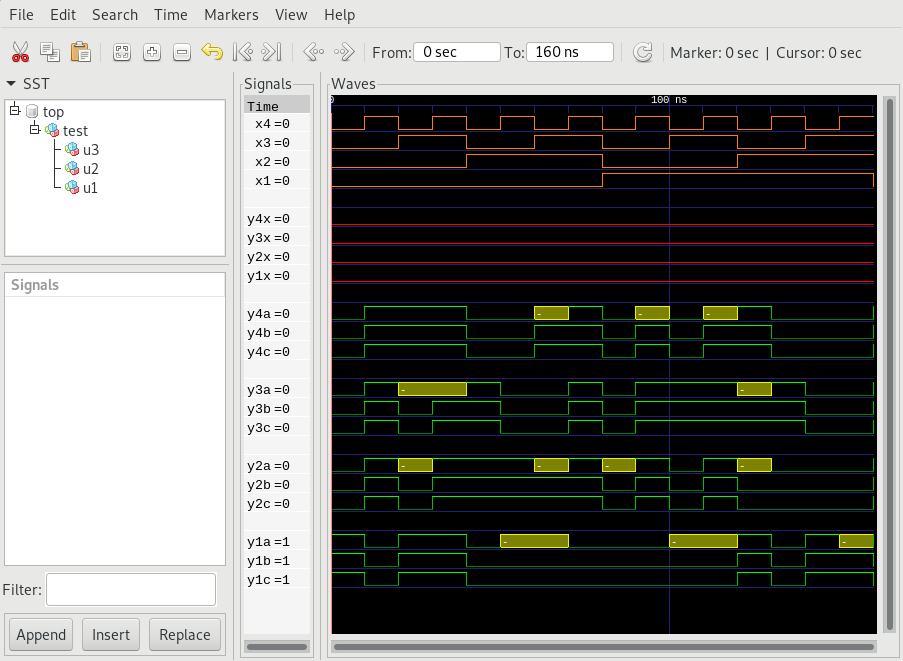
\includegraphics[width=1\textwidth]{figures/overview.png}
    \caption{\textit{Testpingi väljund}}
    \label{fig:wave_overview}
\end{figure}

Joonisel \ref{fig:wave_overview}, \(x_1, x_2, x_3, x_4\) on testpingi sisendid, \(y_1x, y_2x, y_3x, y_4x\) on testpingi väljundid ja signaalid \(y\{_1,_2,_3,_4\}\{a,b,c\}\) on tabeli, espresso ja optimeeritud loogikaskeemi väljundid.

\begin{figure}[ht]
    \centering
    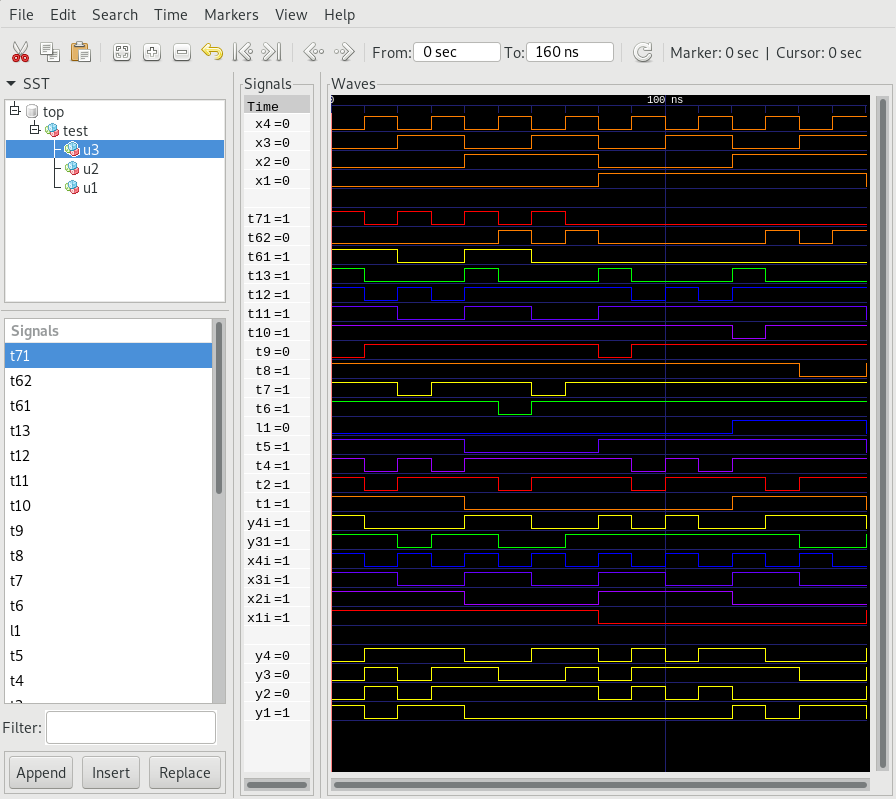
\includegraphics[width=1\textwidth]{figures/opti1.png}
    \caption{\textit{Optimeeritud loogikaskeemi sisemised väärtused}}
    \label{fig:wave_opti1}
\end{figure}

Joonis \ref{fig:wave_opti1} kuvatud signaalid vastavad lisas toodud \verb|opt1o.vhdl| koodile mille listing nr\ref{fs1opt10} leiab lisadest. Joonis \ref{fig:wave_opti1} kuvatud signaalid vastavad lisas toodud \verb|opt1o.vhdl| koodile mille listing nr\ref{fs1opt10} leiab lisadest. 

